\documentclass{beamer}

\usepackage{geometry} % Pour passer au format A4
\usepackage{graphicx} % Required for including pictures
\usepackage{float} % 

\usepackage{amsmath,amsfonts,amssymb,amsthm}
\usepackage[T1]{fontenc} 
\usepackage[english,francais]{babel}
\usepackage[utf8]{inputenc}
\usepackage{lmodern}
\usepackage{eurosym} % signe Euros

\usetheme{Warsaw}

\title{Proportionnalité}
\author{$5^{e}1$}

\begin{document}

\frame{\titlepage}

\section{Proportions}
\subsection{Reconnaître et exploiter une situation de proportionnalité}

\begin{frame}
  \frametitle{Reconnaître et exploiter une situation de proportionnalité}
  \begin{alertblock}{Définition}	
    Deux quantités sont proportionnelles si on peut passer de l'une à l'autre en multipliant par un même nombre non nul : \textbf{le coefficient de proportionnalité}.
  \end{alertblock}

  \begin{block}{Propriété 1}
    Dans un tableau de proportionnalité, on peut additionner des colonnes et multiplier une colonne par un nombre.
  \end{block}
    
  \begin{block}{Propriété 2}
    La représentation graphique de deux quantités proportionnelles est une droite passant par le point 0 de coordonnée (0,0).
  \end{block}
\end{frame}

\subsection{Exemples}

\begin{frame}
  \frametitle{Croissance des bambous}
  \begin{block}{}	
    La croissance des bambous est de 7cm par jours. La taille d'un bambou et son âge sont proportionnels.
    
  \end{block}
  \begin{center}
    \begin{tabular}{| l || c | c | c | c | c |}
      \hline			
      Âge du bambou (en jours) & 1 &  2 &  3 & 10 &  25\\
      \hline  
      Taille du bambou (en cm) & 7 & 14 & 21 & 70 & 175\\
      \hline  
    \end{tabular}
  \end{center}

  \begin{figure}[H]
    \centering
    \includegraphics[width=0.5\linewidth]{sources/cours/bambou.pdf}
  \end{figure}
\end{frame}

\section{Pourcentages}
\subsection{Appliquer un pourcentage}

\begin{frame}
  \frametitle{Appliquer un pourcentage}
  \begin{alertblock}{Définition}	
    Un pourcentage est une fraction avec 100 comme dénominateur. Elle traduit une situation de proportionnalité.
  \end{alertblock}

  \begin{block}{Exemple}
     Un magasin de vêtement propose 20\% de réduction sur un article à 72\euro.\\
  $20\% \text{ de } 72 = \dfrac{20}{100} \times 72 = \dfrac{1440}{100} = 14.4$\euro.\\
  Le prix de l'article après la réduction est : 72 - 14.4 = 57.6\euro.
  \end{block}   
\end{frame}

  \subsection{Rechercher un pourcentage}

\begin{frame}
  \frametitle{Rechercher un pourcentage}
  \begin{alertblock}{Définition}	
    Pour exprimer une proportion sous forme de pourcentage, on écrit la proportion comme une fraction avec 100 comme dénominateur.
  \end{alertblock}

  \begin{block}{Exemple}
     Dans la classe de $5^{e}1$, il y a 25 élèves dont 13 filles et 12 garçons.\\
  $\dfrac{13}{25} = \dfrac{52}{100} = 52 \text{\% de filles et } \dfrac{12}{25} = \dfrac{48}{100} = 48$\% de garçon.
  \end{block}   
\end{frame}

\section{Echelles et temps}
\subsection{Echelles}

\begin{frame}
  \frametitle{Echelles}
      \begin{columns}[t]
      \begin{column}{6cm}
      
    \begin{alertblock}{Définition}	
    L'échelle d'un plan est le quotient à la même unité d'une longueur sur le plan par la longueur réelle qu'elle représente.
  \end{alertblock}

  \begin{block}{Remarque}
    Sur un plan, les longueurs mesurés sont proportionnelles au longueurs qu'elles représentent.
  \end{block}
       \end{column}
      \begin{column}{4cm}  
  \begin{figure}[H]
    \centering
    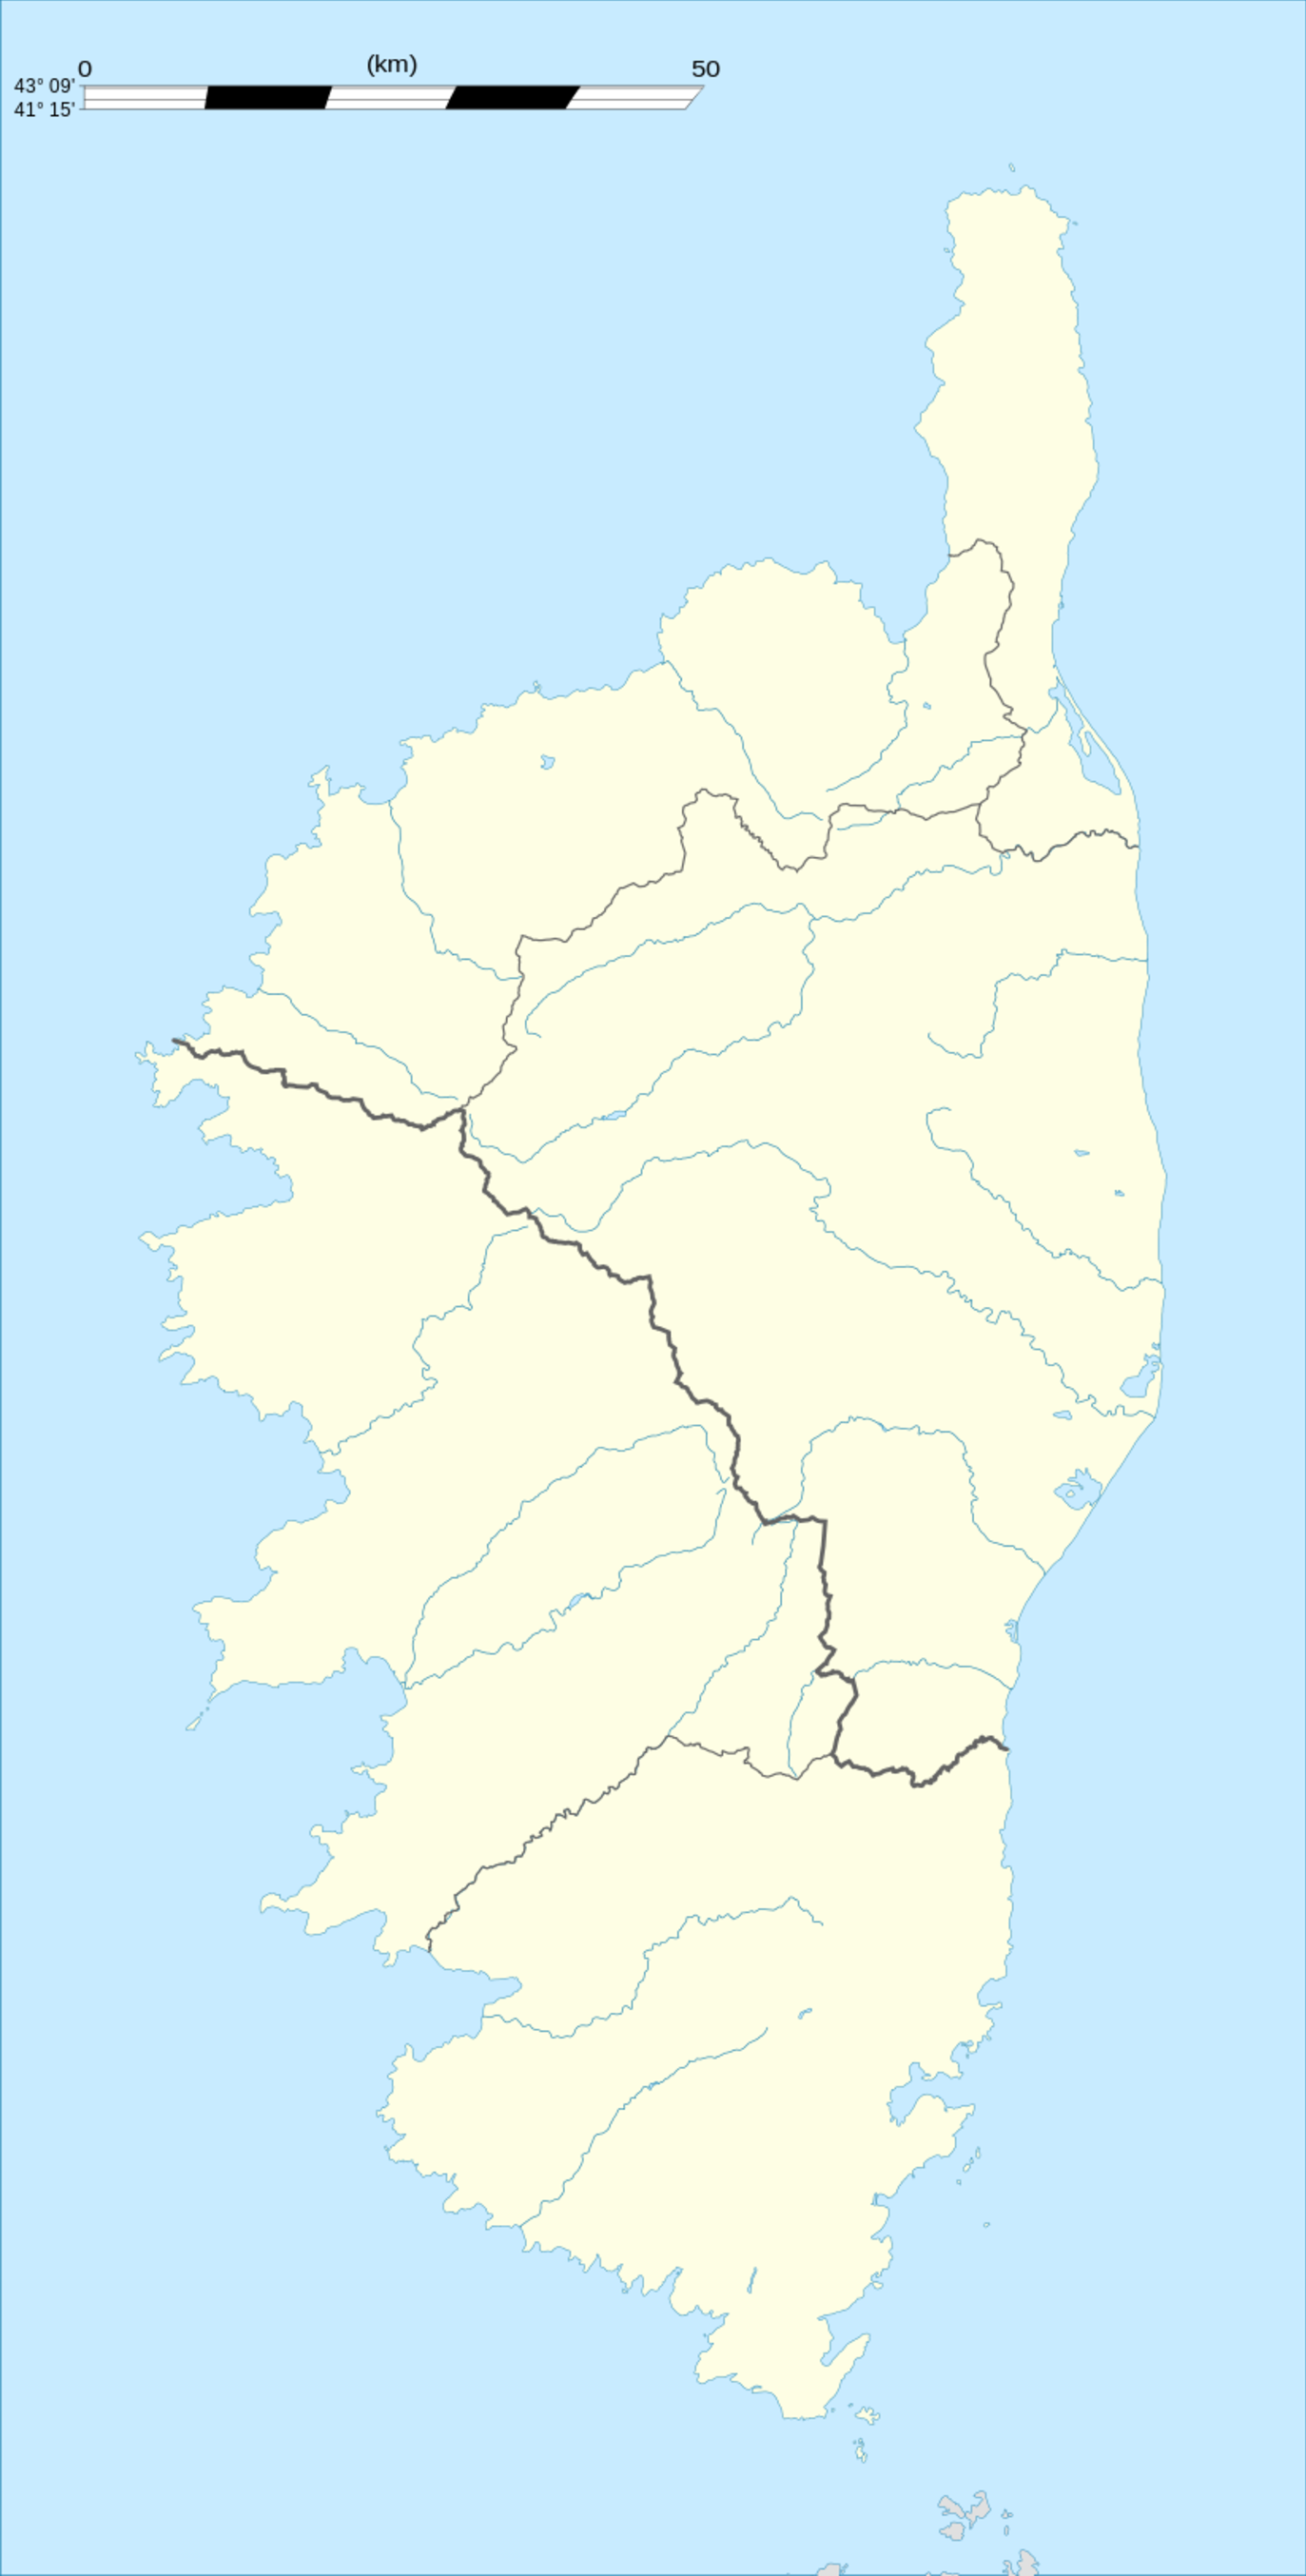
\includegraphics[width=\linewidth]{sources/cours/corse.pdf}
  \end{figure}
        \end{column}
    \end{columns} 
\end{frame}


\subsection{Temps}

\begin{frame}
  \frametitle{Temps}
  \begin{alertblock}{Définition}	
  durée en jours $\stackrel{\times 24}{=}$ durée en heures $\stackrel{\times 60}{=}$ durée en minute $\stackrel{\times 60}{=}$ durée en seconde.
  \end{alertblock}
\end{frame}



\end{document}
